\chapter{Разработка инструмента} \label{ch3}

Предварительно важно определить чёткую последовательность этапов,
которая позволит организовать работу над инструментом системно и управляемо.
Это поможет сократить риски неопределенности, оптимально распределить ресурсы и обеспечить своевременный контроль качества на каждом шаге.

Хорошим стилем является наличие введения к главе. Во введении может быть описана цель написания главы, а также приведена краткая структура главы.

\section{План разработки инструмента} \label{ch3:plan_debeloping}
\begin{enumerate}[label=\textbf{Этап \arabic*.}]
      \item Сбор и анализ требований \\
            На этом этапе формализуются функциональные и нефункциональные требования: определяется, какие компоненты Big Data стека поддерживаются, в каком формате задается исходный YAML, какие конфигурационные артефакты должны генерироваться.
      \item  Проектирование архитектуры \\
            Разрабатывается модульная архитектура инструмента, включающая парсер входного описания, генератор промежуточного представления (AST), набор шаблонов для конфигураций инструментов и механизм их объединения в итоговые файлы. Определяются границы ответственности каждого модуля, протокол взаимодействия между ними и формат плагинов для расширения функциональности.
      \item  Определение языка декларативного описания \\
            Уточняются синтаксис и семантика входного YAML: структура разделов, типы параметров, возможные зависимости и проверки корректности. Разрабатывается схема jsonschema для валидации пользовательских описаний на раннем этапе.
      \item  Реализация ядра: парсер и промежуточное представление \\
            Пишется компонент, который читает декларативный файл, проводит его валидацию по схеме (jsonschema), конструирует внутреннее дерево объектов (AST) с отображением всех сущностей и их связей. Этот модуль обеспечивает основу для дальнейших операций по генерации конфигураций.
      \item Разработка генераторов конфигурационных файлов \\
            На основе AST реализуются плагины-генераторы для каждого типа артефакта:
            \begin{itemize}
                  \item docker-compose.yaml с сервисами и сетями;
                  \item Конфигурации PostgreSQL (postgresql.conf, init.sql);
                  \item JSON-файлы коннекторов Debezium и S3Sink;
                  \item Файлы настроек для ClickHouse;
                  \item Конфигурационные файлы для AKHQ и Superset.
            \end{itemize}
            Каждый генератор использует шаблонизатор и преобразует параметры из AST в конкретные строки и блоки файлов.
      \item Создание CLI-интерфейса\\
            Реализуется утилита командной строки, позволяющая пользователю запускать генерацию: передавать путь к входному файлу,  указывать директорию вывода, включать опции валидации и отладки. CLI обеспечивает удобство использования инструмента в скриптах и CI/CD-пайплайнах\cite{acid}.
      \item Модуль тестирования и валидации\\
            Пишутся автоматические тесты: модульные тесты для парсера и генераторов, интеграционные — для проверки корректного результата генерации по ряду типовых YAML-конфигураций. Добавляются проверки на соответствие с эталонными файлами и на корректность в Docker-среде (например, пробный запуск docker-compose up).
      \item Документирование и примеры\\
            Готовится подробная документация: описание формата входного файла, руководство пользователя CLI, схемы и примеры конфигураций «из коробки» для типовых сценариев (EDW на PostgreSQL→Kafka→ClickHouse→Superset). Включаются рекомендации по расширению и отладке.
      \item Пилотное развертывание и сбор обратной связи\\
            Инструмент разворачивается в тестовой среде или локально на реальных примерах, собираются отзывы от пользователей — инженеров и аналитиков. На основе полученных замечаний корректируются шаблоны, схемы и UX CLI.
      \item Релиз и сопровождение\\
            Формируется релизная сборка, обеспечивается публикация в открытый репозиторий GitHub, настраивается процесс выпуска обновлений и приёма issue. Определяется модель поддержки: дорожная карта, приоритеты новых возможностей и исправлений.
\end{enumerate}


\section{Язык декларативного описания (DSL)} \label{ch3:dsl}
Практический опыт показывает, что повышение уровня абстракции и учёт специфики предметной области наиболее эффективно достигаются через разработку собственного языка предметной области - Domain Specific Language, DSL\cite{novikov_grammatik}\cite{ulman}. Такой язык представляет собой формальный аппарат, работающий непосредственно с понятиями и структурами предметной области, позволяя лаконично формулировать и решать большинство типовых задач.

В нашем случае DSL строится на основе YAML\cite{yaml} – удобного человеко-ориентированного формата сериализации, концептуально схожего с языками разметки, но оптимизированного для записи и чтения распространённых структур данных.


Ключевые особенности синтаксиса YAML:
\begin{enumerate}[1.]
      \item Отступы и вложенность\\
            Используются только пробелы (обычно 2 или 4) для обозначения уровней вложенности. Символ табуляции запрещён.
      \item Пары «ключ–значение»\\
            Каждая запись имеет вид ключ: значение, где после двоеточия обязательно идёт пробел.
      \item Списки\\
            Элементы маркируются дефисом и пробелом (- элемент).
      \item Многострочные литералы\\
            Символ | сохраняет все разрывы строк. Символ > объединяет строки, заменяя отступы и разрывы единичными пробелами.
      \item Якоря и ссылки\\
            Якорь (\&имя) позволяет дать имя блоку значений. Ссылка (*имя) повторно вставляет ранее объявленный блок.\\
            Пример:
\end{enumerate}

\begin{verbatim}
        default: &base
        имя: Oleg
        возраст: 27

        user_2:
        <<: *base
\end{verbatim}
Чтобы формализовать синтаксис DSL и задать конечное описание потенциально
бесконечного множества допустимых конфигураций,
мы опираемся на контекстно-свободную грамматику $G=\langle N,T,R,S\rangle$, где:\\
$N$ – множество нетерминальных символов \\
$T$ – терминальные (т. е. реальные лексемы) \\
$R$ – правило вида $A$→$\alpha$ (замена нетерминала A на строку символов $\alpha$) \\
$S$ – стартовый нетерминал.

По классификации Хомского такая грамматика относится ко второму типу (КСГ): в каждом правиле слева стоит ровно один нетерминал, который может быть заменён на любую допустимую цепочку из  $A\cup B$.

Реализация парсера и генератора AST (абстрактного синтаксического дерева) опирается на ANTLR (ANother Tool for Language Recognition)\cite{antlr_lab}.
Лексические правила (начинаются с большой буквы) описывают, как разбить входной текст на токены.
Пример:\\
\begin{verbatim}
// Лексическое правило для целых чисел
INT : [0-9]+ ; 
\end{verbatim}
Синтаксические правила (начинаются с маленькой буквы) задают структуры из токенов.
Пример:
\begin{verbatim}
// Синтаксическое правило для списка аргументов
args : expr (',' expr)* ; 
\end{verbatim}
Для группировки, повторений и альтернатив в ANTLR применяются:\\
«()» – группировка\\
«*» – 0 или более повторений\\
« +» – 1 или более\\
«?» – 0 или 1 раз\\
« |» – выбор одной из альтернатив\\
«:» и «;» – разделители начала и конца правил.\\

Описание языка DPD (Data Platform Deployer)

Язык DPD  разработан для  декларативного описания архитектуры платформы данных единым удобным форматом и автоматической генерации всех необходимых инструментов для быстрого развертывания и тестирования готового стенда. В общих чертах имеет следующую структуру:
\begin{verbatim}
project:
    name: data-platform-14
    version: 1.2.0
    description: This is a project for testing data platform
sources:
    - type: postgres
    name: postgres_1
    - type: postgres
    name: postgres_2
    - type: s3
    name: s3_1
streaming:
    kafka:
        num_brokers: 3
    connect:
        name: connect-1
storage:
    clickhouse:
    name: clickhouse-1
bi:
    superset:
    name: superset-1
\end{verbatim}
В приложении \ref{grammatic-dpd}  приведена часть полной грамматики, описывающая правила в форме ANTLR \\



% \FloatBarrier % заставить рисунки и другие подвижные (float) элементы остановиться


\section{Описание процесса автогенерации конфигураций программных систем платформы данных} \label{ch3:process_generation}
Архитектура инструмента в значительной степени повторяет логическое разбиение на блоки, которое представлено в начале этой главы.

Пакет \texttt{data platform} взаимодействует с пакетом \texttt{core}, внутри которого как раз таки находятся парсер, генератор, сервисы, а также другие дополнительные элементы.
Диаграмма представлена на рисунке \ref{fig:diagram_package}

\begin{figure}
      \center
      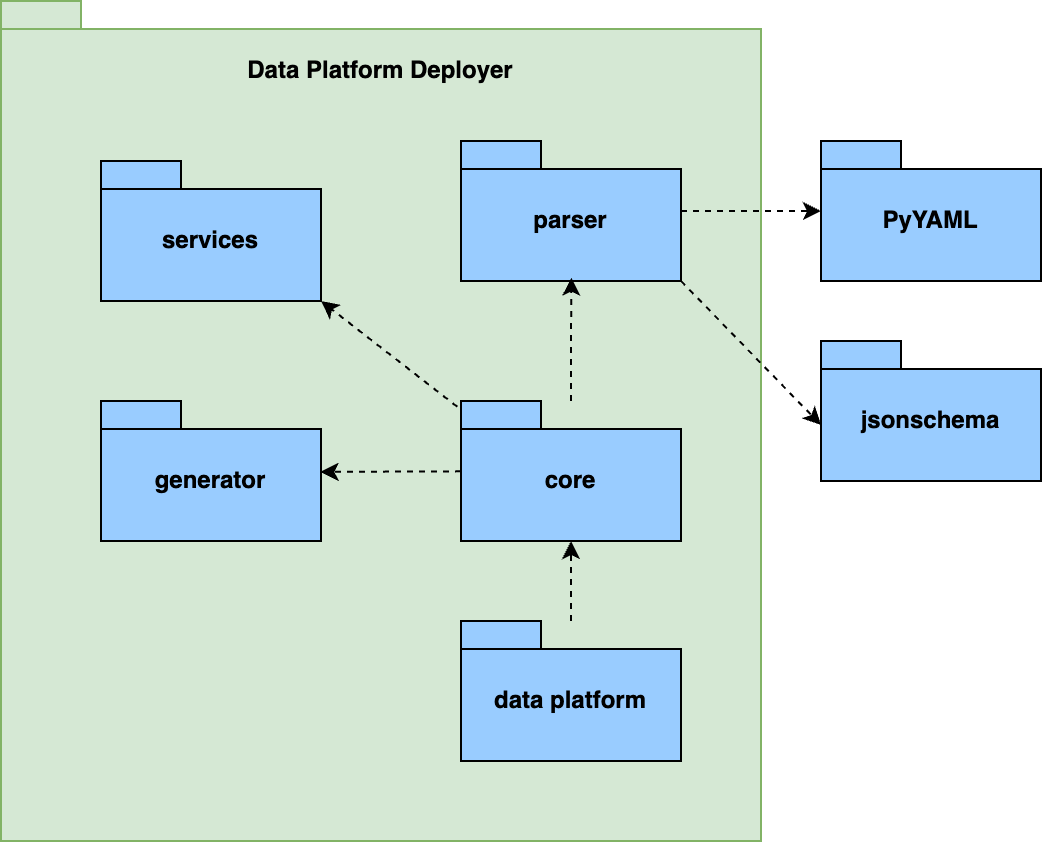
\includegraphics [scale=0.4] {my_folder/images/diagram_package}
      \caption{Диаграмма пакетов}
      \label{fig:diagram_package}
\end{figure}
\FloatBarrier
Стоит детальнее рассмотреть содержимое пакета \texttt{core}, ведь именно там выполняется генерация конфигураций программных систем платформы данных.
Процесс автоматической генерации конфигураций для платформы данных с использованием инструмента \texttt{dpd} можно разделить на следующие ключевые этапы:
\begin{enumerate}[1.]

      \item Инициация через командную строку (\texttt{main.py})
            \begin{itemize}
                  \item \textbf{Входная точка.} Пользователь взаимодействует с инструментом через CLI, вызывая основную команду \texttt{dpd}.
                  \item \textbf{Команда \texttt{generate}.} Логика запускается командой
                        \texttt{dpd generate} с обязательным параметром
                        \texttt{--config <путь\_к\_YAML>}.
                  \item \textbf{Оркестрация.} Файл \texttt{main.py} парсит аргументы командной строки, вызывает функции валидации и загрузки конфигурации, инициализирует генератор платформы и запускает процесс, выводя информативные сообщения.
            \end{itemize}

      \item Валидация и загрузка конфигурации (\texttt{main.py} \textrightarrow\ \texttt{dpd.models}):
            \begin{itemize}
                  \item \textbf{Проверка схемы.} Перед генерацией выполняется валидация YAML-конфига по JSON-схеме (\texttt{src/dpd/schema.json}) с помощью функции \texttt{validate} из \texttt{dpd.models} и библиотеки \texttt{jsonschema}.
                  \item \textbf{Загрузка и моделирование.} При успешной валидации содержимое конфигурации загружается и преобразуется в Python-модели (\texttt{Config}, \texttt{Postgres}, \texttt{S3} и т.~п.) через функцию \texttt{load\_config\_from\_file}.
            \end{itemize}

      \item Инициализация генератора платформы (\texttt{main.py} \textrightarrow\ \texttt{data\_platform.py})
            \begin{itemize}
                  \item \textbf{Создание \texttt{DPGenerator}.} В конструктор передаётся смоделированная конфигурация (\texttt{conf}).
                  \item \textbf{Начальное состояние.} Генератор инициализирует пустые словари для сервисов и настроек, создаёт описание сетей Docker на основе имени проекта, подготавливает \texttt{PortManager} и \texttt{EnvManager}.
            \end{itemize}

      \item Обработка сервисов и делегирование (\texttt{DPGenerator.process\_services})
            \begin{itemize}
                  \item \textbf{Итерация.} Метод перебирает секции конфигурации (\texttt{sources}, \texttt{streaming}, \texttt{storage}, \texttt{bi}).
                  \item \textbf{Делегирование.} В зависимости от компонента (\texttt{postgres}, \texttt{s3}, \texttt{kafka}, \texttt{clickhouse}, \texttt{superset}) вызываются соответствующие статические методы \texttt{generate()} из модулей \texttt{dpd.services}.
                  \item \textbf{Сборка.} Каждый сервис генерирует свой блок для \texttt{docker-compose.yml} и вспомогательные файлы, результат добавляется в словарь \texttt{self.services}.
                  \item \textbf{Зависимости.} Для некоторых генераций (например, \texttt{KafkaConnectService}) учитываются заранее созданные компоненты (Postgres-источники и т.~п.).
            \end{itemize}

      \item Генерация вспомогательных файлов
            \begin{itemize}
                  \item \textbf{README.md.} \texttt{ReadmeService.generate\_file()} создаёт описание платформы и инструкции.
                  \item \textbf{.env.} \texttt{EnvManager.generate\_env\_file()} помещает все секреты (пароли, ключи) в файл \texttt{.env}.
                  \item \textbf{init.sql.} \texttt{PostgresqlService.generate\_init\_sql\_script()} формирует SQL-скрипт для инициализации (создание публикации, репликационные слоты).
                  \item \textbf{postgresql.conf.} \texttt{PostgresqlService.generate\_conf\_file()} генерирует конфигурацию WAL (напр., \texttt{wal\_level}, \texttt{max\_wal\_senders}, \texttt{max\_replication\_slots}).
                  \item \textbf{Конфигурации Debezium и S3SinkConnector.} Функции \texttt{generate\_debezium\_configs()} и \texttt{generate\_s3sink\_configs()} создают JSON-файлы для репликации Postgres→Kafka и Kafka→S3, которые затем загружаются в Kafka Connect через REST API.
                  \item \textbf{Плагины для Kafka Connect.} Автоматически скачиваются JAR-файлы S3SinkConnector и ClickHouseConnector.
                  \item \textbf{AKHQ.} \texttt{KafkaUIService.generate\_conf\_file()} связывает веб-интерфейс AKHQ с кластерами Kafka и Kafka Connect.
            \end{itemize}

      \item Сборка и запись итогового файла
            \begin{itemize}
                  \item \textbf{Формирование структуры.} Метод \texttt{generate()} собирает все настройки, описания сервисов, тома (метод \texttt{\_generate\_volumes()}) и сети в единый Python-словарь, соответствующий формату \texttt{docker-compose.yml}.
                  \item \textbf{Сериализация.} Структура преобразуется в YAML при помощи \texttt{PyYAML}.
                  \item \textbf{Запись.} Итоговый YAML записывается в файл \texttt{docker-compose.yml} в директории с именем проекта. Директория создаётся автоматически при необходимости.
            \end{itemize}
\end{enumerate}

Таким образом, инструмент \texttt{dpd} берёт на вход декларативное описание платформы данных, проверяет его, последовательно генерирует конфигурации для каждого компонента и собирает их в готовый к запуску стек под управлением Docker Compose, а также создаёт сопутствующие файлы (\texttt{README.md}, \texttt{.env}, \texttt{postgresql.conf}, \texttt{dbz\_conf.json}, \texttt{s3\_sink.json}, \texttt{akhq\_conf.yml} и др.).


% Текст выводов по главе \thechapter.


%% Вспомогательные команды - Additional commands
%
%\newpage % принудительное начало с новой страницы, использовать только в конце раздела
%\clearpage % осуществляется пакетом <<placeins>> в пределах секций
%\newpage\leavevmode\thispagestyle{empty}\newpage % 100 % начало новой страницы